%%%%%%%%%%%%%%%%%%%%%%%%%%%%%%%%%%%%%%%%%%%%%%%%%%%
%
%  New template code for TAMU Theses and Dissertations starting Fall 2012.  
%  For more info about this template or the 
%  TAMU LaTeX User's Group, see http://www.howdy.me/.
%
%  Author: Wendy Lynn Turner 
%	 Version 1.0 
%  Last updated 8/5/2012
%
%%%%%%%%%%%%%%%%%%%%%%%%%%%%%%%%%%%%%%%%%%%%%%%%%%%
%%%%%%%%%%%%%%%%%%%%%%%%%%%%%%%%%%%%%%%%%%%%%%%%%%%%%%%%%%%%%%%%%%%%%%
%%                           SECTION III
%%%%%%%%%%%%%%%%%%%%%%%%%%%%%%%%%%%%%%%%%%%%%%%%%%%%%%%%%%%%%%%%%%%%%



\chapter{\uppercase{Fuel Depletion Problem}}
\label{sec:chapter5_depletion}

\section{Specfication}


We consider a fuel depletion problem to illustrate that self-lumping DFEM schemes remain accurate for more complex physics than simply a purely absorbing medium.
The depletion method we use [time stepping scheme, time step size, etc.] is chosen for its simplicity, not for its fidelity relative to state-of-the art depletion methodologies.  
Our goal is to assess the accuracy of {\emph spatial discretization} methods for problems with spatially varying cross sections, not to propose a new depletion method.  
However, we stress that self-lumping methods can be implemented with any time depletion method or time stepping scheme since implementation of self-lumping  only requires changes pertaining to the spatial discretization. Indeed,  a depletion scheme that uses a cell-wise constant cross section at a given time $t^\ast$ computes the interaction matrix 
as
\benum
\mathbf{R}_{\hat \Sigma^*} =  \hat{\Sigma}^* \mathbf{M} \pep
\eenum
With self-lumping, one would only need to use the space-dependent cross section at the same time to obtain
\benum
(\mathbf{R}_{\Sigma^*})_{ij} =  \left \{ \begin{array}{ll}
w_i \Sigma^*(s_i) ~ & ~ i=j \\
 0 & ~\text{otherwise}
\end{array}
\right. 
\pep
\eenum

The complete definition and detailed solution methodology for the fuel depletion problem are provided in %\appref{app:depletion}.  
The 1-D geometry of fuel and moderator layers is shown in \fig{fig:lattice}.  
\begin{figure}[!htp]
\begin{center}
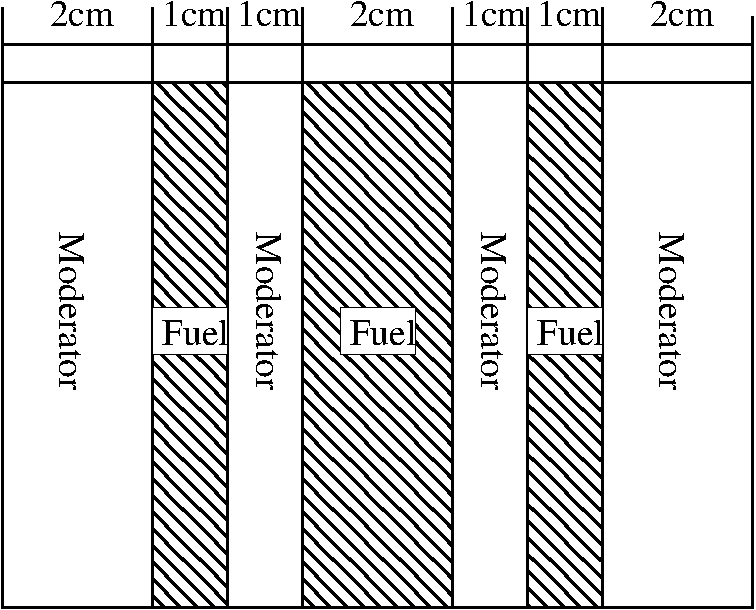
\includegraphics[width=8cm]{chapter5_depletion/article_grid.pdf}
\end{center}
\caption{Depletion problem fuel/moderator lattice.}
\label{fig:lattice}
\end{figure}
The fresh fuel composition is spatially uniform in each fuel region.
As the fuel depletes, its isotopic concentrations will deviate from being cell-wise constant.
We track five nuclide densities in  each fuel region:
\begin{enumerate}
\item fissile $(N_{FS})$,
\item fertile $(N_{FT})$,
\item parasitic absorber fission product $(N_{FP-A})$,
\item scattering fission product $(N_{FP-S})$, and
\item inert $(N_I)$.
\end{enumerate}
Each fuel region is initially loaded only with fissile and fertile nuclides.  
We assume no radioactive decay.
All possible transmutation paths are shown in \fig{fig:transmutation}.
\begin{figure}[!htp]
\begin{center}
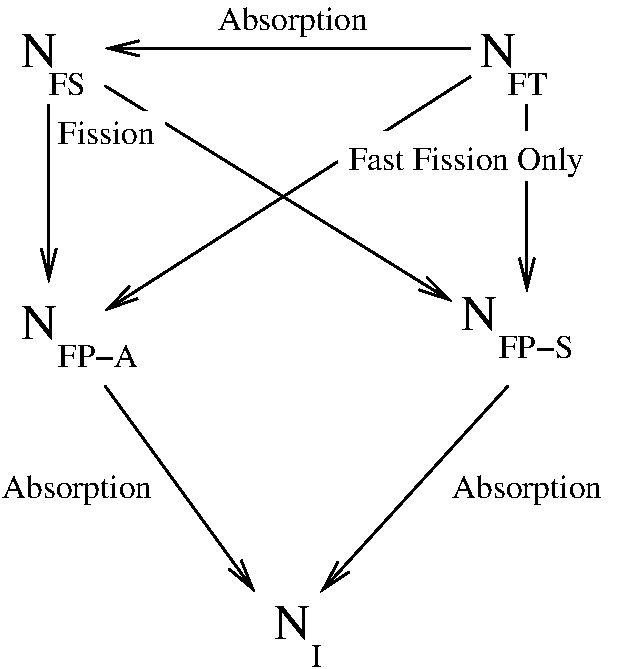
\includegraphics[width=8cm]{chapter5_depletion/article_transmutation.pdf}
\end{center}
\caption{Depletion problem possible transmutation paths and mechanisms.}
\label{fig:transmutation}
\end{figure}
Vacuum boundary conditions are imposed on both sides of the slab.  
We normalize reactor scalar flux values so that the reactor produces a constant fission power level of $2000~[W]$ for the duration of the burn-up cycle.
The burn-up cycle length consists of 600 full-power days and we use a time step of 10 days to update the scalar fluxes.
A typical beginning-of-cycle flux profile is shown in \fig{fig:ex_boc_cycle} and an end-of-cycle scalar flux profile is shown in \fig{fig:ex_eoc_cycle}.  
\begin{figure}[!htp]
\centering
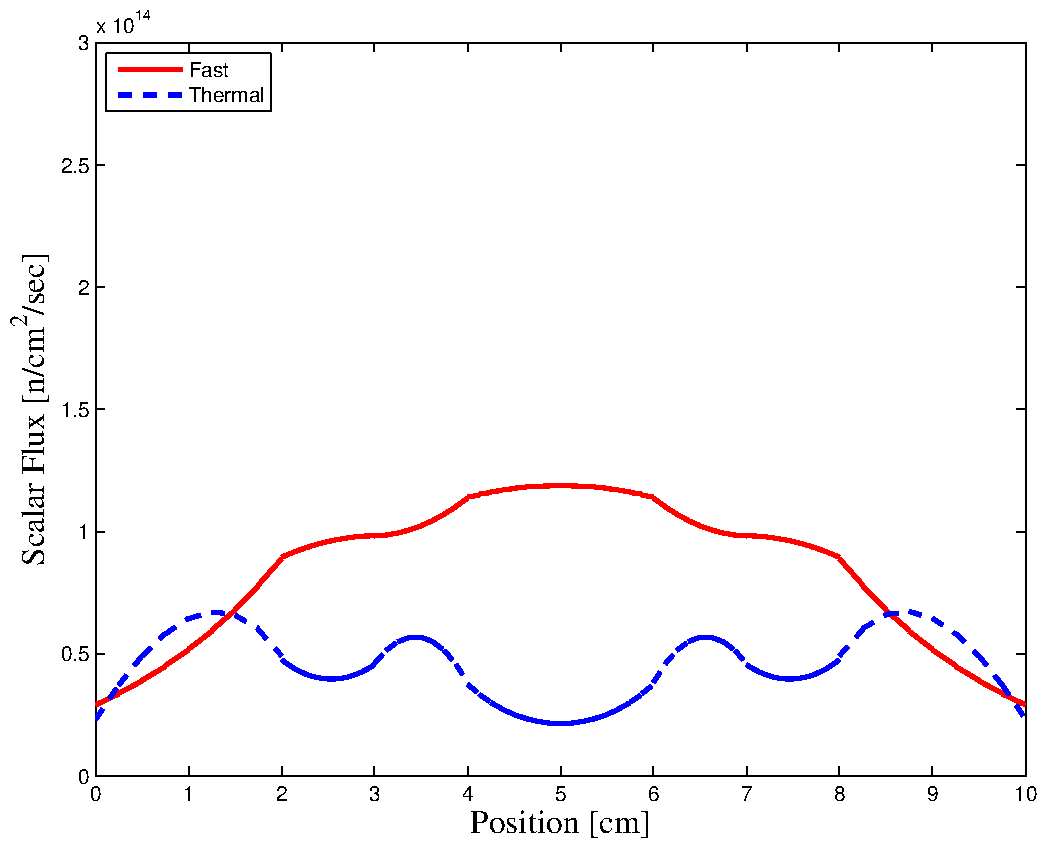
\includegraphics[width=10cm]{chapter5_depletion/P1_Lobatto_full_80_cells_t_steps60_End_600_Power_2000__BOC_Flux.pdf}
\caption{Example normalized scalar flux profiles at beginning and end of fuel burn-up cycle.}
\label{fig:ex_boc_cycle}
\end{figure}

\begin{figure}[!hbp]
\centering
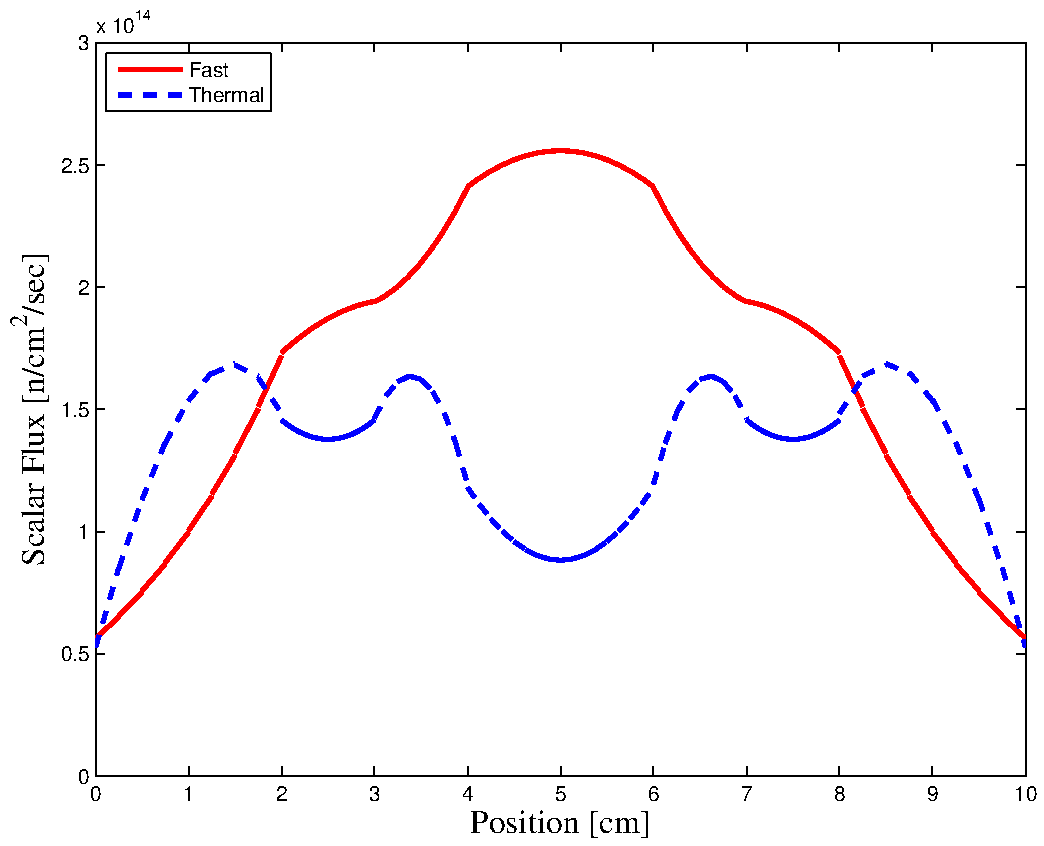
\includegraphics[width=10cm]{chapter5_depletion/P1_Lobatto_full_80_cells_t_steps60_End_600_Power_2000__EOC_Flux.pdf}
\caption{Example normalized scalar flux profiles at beginning and end of fuel burn-up cycle.}
\label{fig:ex_eoc_cycle}
\end{figure}
%For all calculations, we use an $S_2$ Gauss quadrature to discretize in angle.
We consider three numerical methods,
\begin{enumerate}
\item SL Full: expand both the angular flux and nuclide densities in a degree $P$ DFEM trial space, compute $\mathbf{R}_{\Sigma_t}$ as in \eqt{eq:chap3_sl_react}, and $\mathbf{M}$ as in \eqt{eq:self_lump_def};
\item SL Collapse: expand both the angular flux and nuclide density in a degree $P$ DFEM trial space, but compute $\mathbf{R}_{\Sigma_t}$ assuming a cell-wise constant cross section and self-lumping quadrature to approximate $\mathbf{M}$ as in \eqt{eq:self_lump_def}; and
\item AD DFEM: expand the angular flux in a $P$ degree polynomial DFEM trial space, track only the cell average nuclide density, exactly integrate $\mathbf{M}$, and use a cell-wise average cross section as in \eqt{eq:chap3_cxs_R} to compute $\mathbf{R}_{\Sigma_t}$.
\end{enumerate}
The SL Full and SL Collapse schemes use a Lobatto quadrature for the DFEM interpolation points for odd degree polynomial trial spaces and a Gauss quadrature for  interpolation points when the DFEM trial space is an even degree polynomial.
The choice of interpolation type does not affect the numerical results of the AD DFEM scheme.
SL Collapse expands the nuclide density in a $P$ degree polynomial for the purpose of advancing the nuclide production/destruction equations but uses a cell-wise average cross section for updating the scalar flux.  
Given the DFEM approximation, $\widetilde{N}(x)$, to the true nuclide density, $N(x)$, SL Collapse calculates $\hat{\Sigma}_t$ for each cell, using the cell average of $\widetilde{N}(x)$ to generate an average cross section for each cell to update the scalar flux.

Since an analytic solution to this depletion problem is not available we employ a fine spatial mesh to obtain the reference solution.  
We use a fine mesh of 10,240 cells and the SL Full scheme with a quartic polynomial trial space as our reference numerical solution. 
%Our results demonstrate that the SL Full scheme using a quartic polynomial DFEM trial space is the most accurate scheme.   
We present $L_2$ spatial error measures for 
\begin{enumerate}
\item the total scalar flux ($E_{\phi}$), 
\item the fissile nuclide density ($E_{N_{FS}}$),
\item the fertile nuclide density ($E_{N_{FT}}$), and 
\item the parasitic absorber fission product ($E_{N_{FP-A}}$).
\end{enumerate}
To allow for easier comparison, we normalize each error to the reference solution quantity.
We define $E_{\phi}$ as:
\benum
E_{\phi} = \frac{\sqrt{\sum_{g=1}^2{\sum_{i=1}^{N_{ref}}{ \frac{\Delta x_i}{2} \sum_{q=1}^{N_{qf}}{ w_q\left( \widetilde{\phi}_{ref,i,g}(s_q) - \widetilde{\phi}_{num,i,g}(s_q)  \right)^2}}}}}{\sqrt{\sum_{g=1}^2{\sum_{i=1}^{N_{ref}}{ \frac{\Delta x_i}{2} \sum_{q=1}^{N_{qf}}{ w_q\widetilde{\phi}_{ref,i,g}(s_q)^2  }}}}} \pec
\eenum
%
%
%%%E_{N_{FS}} &=& \frac{\sqrt{\sum_{i=1}^{N_{ref}}{ \frac{\Delta x_i}{2} \sum_{q=1}^{N_{qf}}{ w_q\left( \widetilde{N}_{FS,ref,i}(s_q) - \widetilde{N}_{FS,num,i}(s_q)  \right)^2}}}}{\sqrt{\sum_{i=1}^{N_{ref}}{ \frac{\Delta x_i}{2} \sum_{q=1}^{N_{qf}}{ w_q\widetilde{N}_{FS,ref,i}(s_q)^2  }}}} \pec \\
%%%%
%%%%
%%%E_{N_{FT}} &=& \frac{\sqrt{\sum_{i=1}^{N_{ref}}{ \frac{\Delta x_i}{2} \sum_{q=1}^{N_{qf}}{ w_q\left( \widetilde{N}_{FT,ref,i}(s_q) - \widetilde{N}_{FT,num,i}(s_q)  \right)^2}}}}{\sqrt{\sum_{i=1}^{N_{ref}}{ \frac{\Delta x_i}{2} \sum_{q=1}^{N_{qf}}{ w_q\widetilde{N}_{FT,ref,i}(s_q)^2  }}}} \pec \\
%%%%
%%%%
%%%E_{N_{FP-A}} &=& \frac{\sqrt{\sum_{i=1}^{N_{ref}}{ \frac{\Delta x_i}{2} \sum_{q=1}^{N_{qf}}{ w_q\left( \widetilde{N}_{FP-A,ref,i}(s_q) - \widetilde{N}_{FP-A,num,i}(s_q)  \right)^2}}}}
%%%{\sqrt{\sum_{i=1}^{N_{ref}}{ \frac{\Delta x_i}{2} \sum_{q=1}^{N_{qf}}{ w_q\widetilde{N}_{FP-A,ref,i}(s_q)^2  }}}} \pep
%%%\eeanum
where $N_{ref}$ is the number of reference cells, $\widetilde{\phi}_{ref,i,g}(s)$ is the reference solution group $g$ scalar flux in cell $i$, and $\widetilde{\phi}_{num,i,g}(s)$ is the coarse mesh numerical scheme's approximation of the group $g$ scalar flux in cell $i$.
Error measures for $N_{FS}$, $N_{FT}$, and $N_{FP-A}$ are derived similarly.

Convergence of $E_{\phi}$ is shown in \figs{fig:depletion_flux_p1}{fig:depletion_flux_p4} as a function of DFEM trial space degree and DFEM scheme.
\begin{figure}[!htp]
\centering
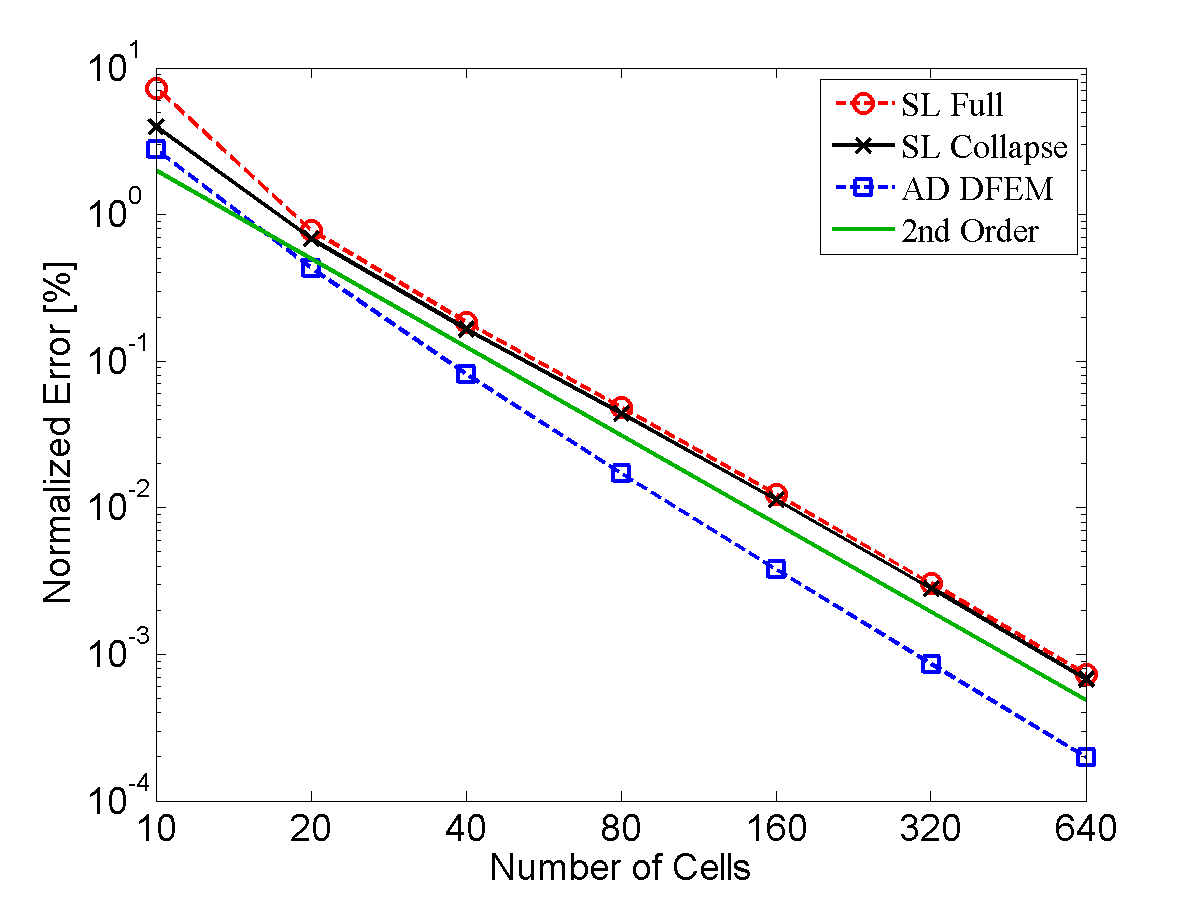
\includegraphics[width=11cm]{chapter5_depletion/Flux_P1_norm_err.png}
\caption{Normalized total scalar flux error, $E_{\phi}$, for the depletion problem at end of cycle, as a function of angular flux trial space degree.}
\label{fig:depletion_flux_p1}
\end{figure}

\begin{figure}[!hbp]
\centering
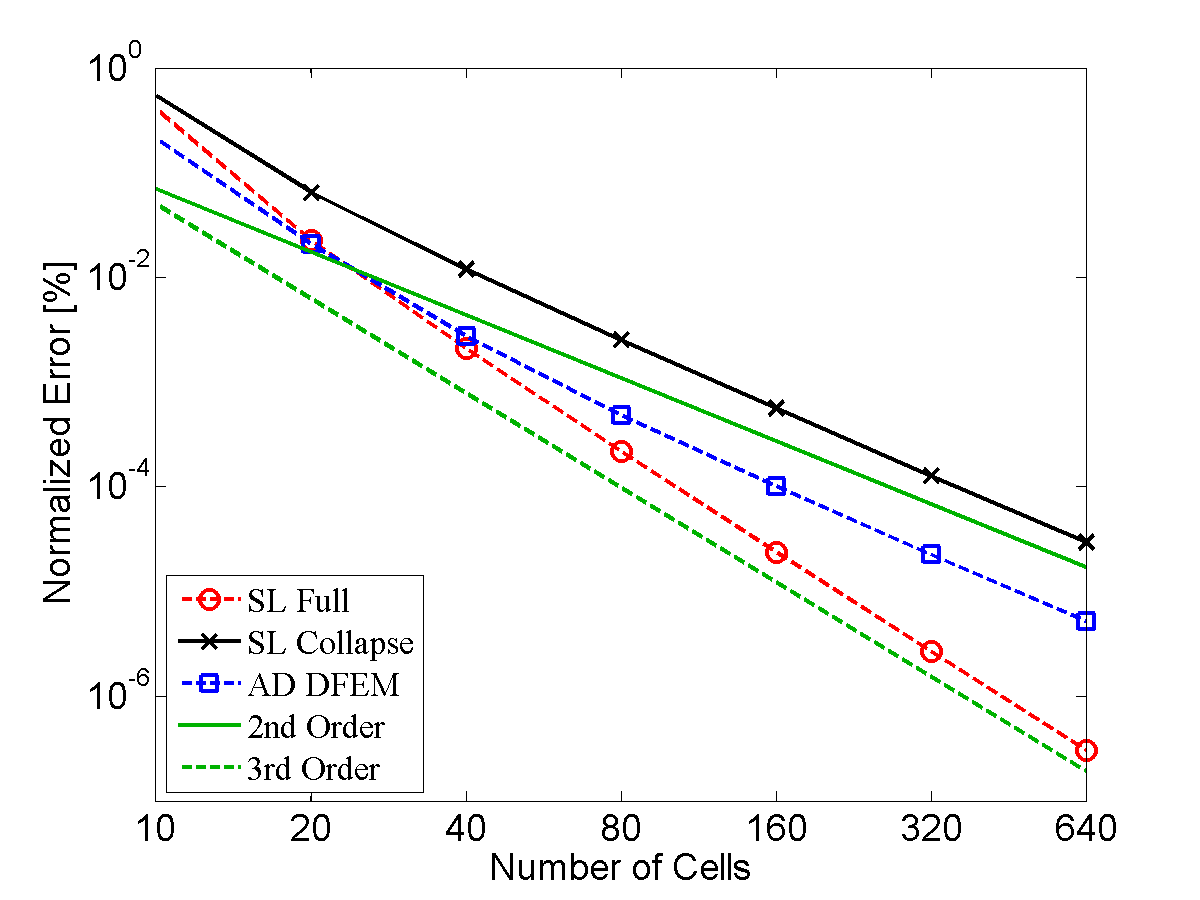
\includegraphics[width=11cm]{chapter5_depletion/Flux_P2_norm_err.png}
\caption{Normalized total scalar flux error, $E_{\phi}$, for the depletion problem at end of cycle, as a function of angular flux trial space degree.}
\label{fig:depletion_flux_p2}
\end{figure}

\begin{figure}[!htp]
\centering
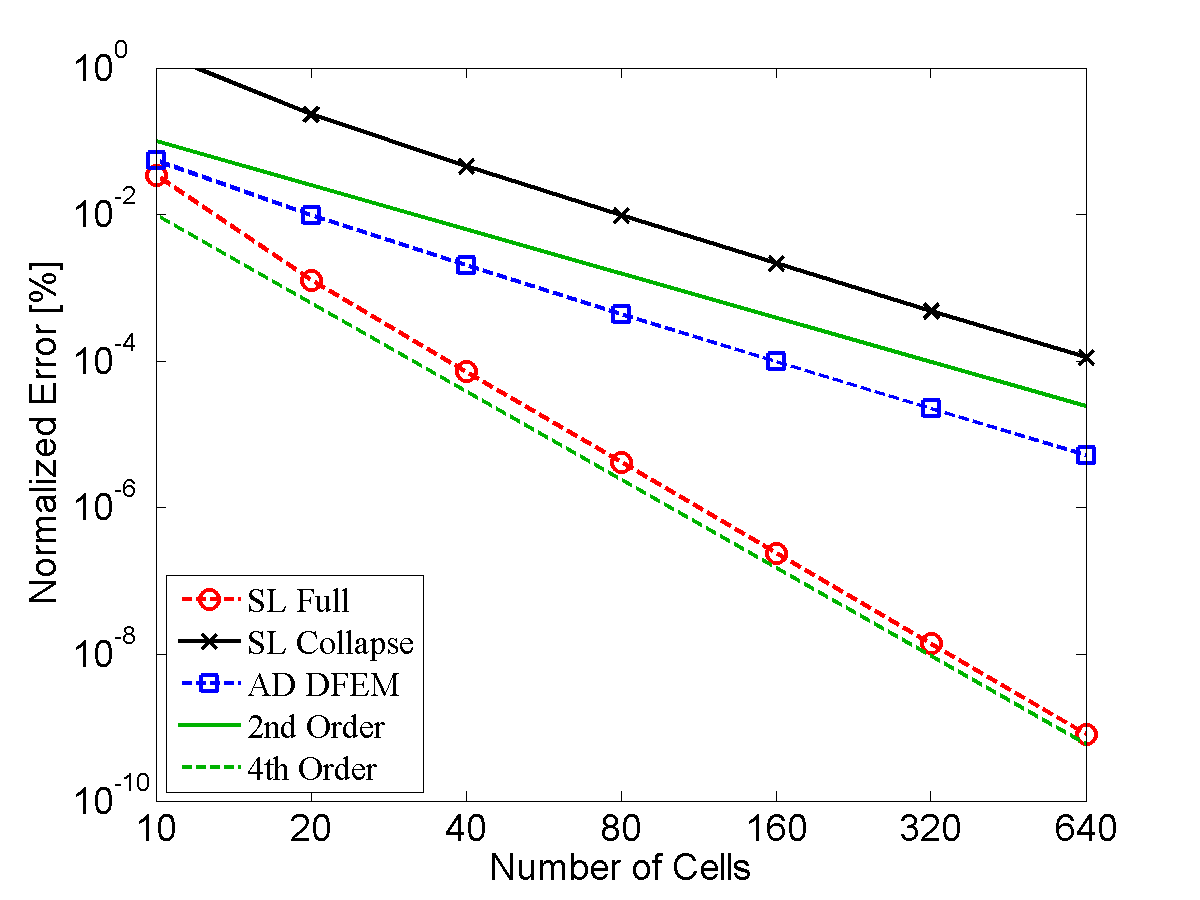
\includegraphics[width=11cm]{chapter5_depletion/Flux_P3_norm_err.png}
\caption{Normalized total scalar flux error, $E_{\phi}$, for the depletion problem at end of cycle, as a function of angular flux trial space degree.}
\label{fig:depletion_flux_p3}
\end{figure}

\begin{figure}[!hbp]
\centering
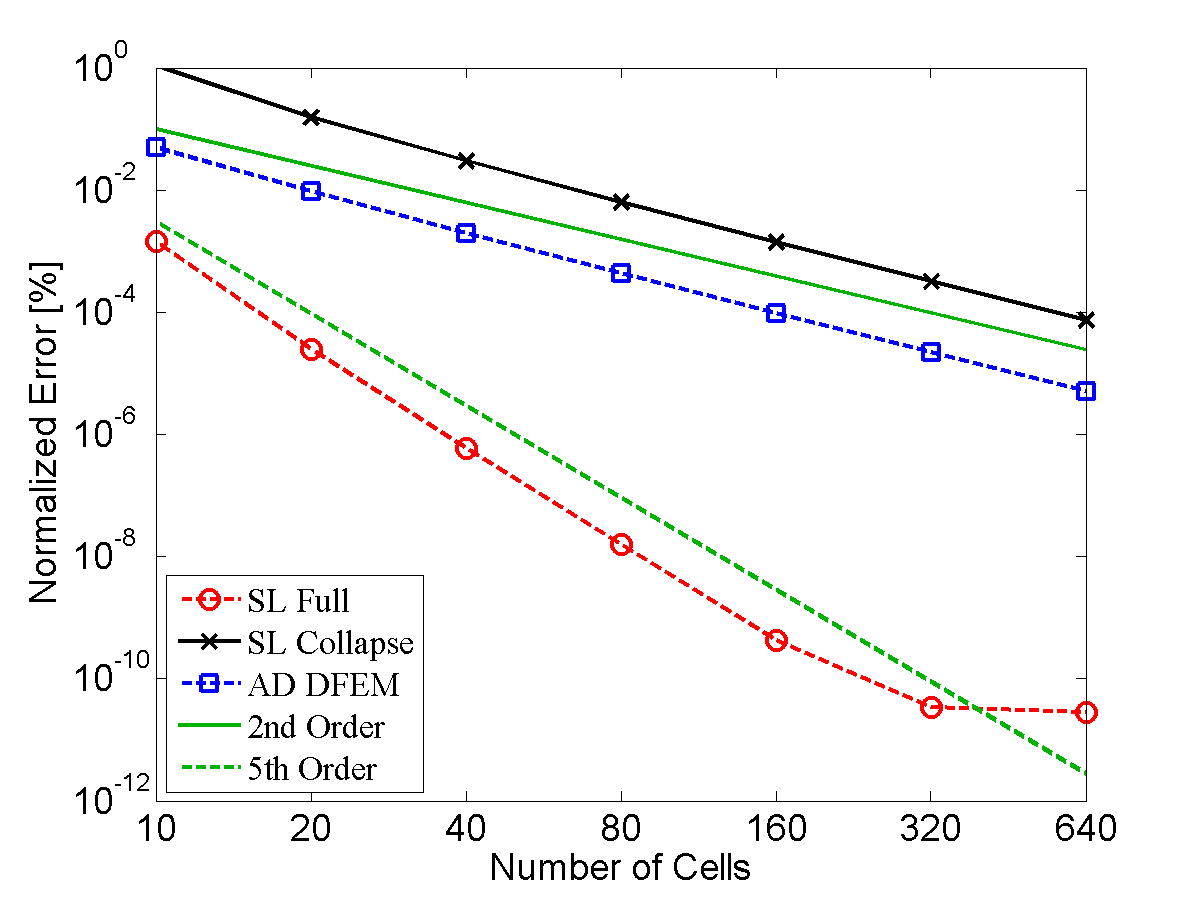
\includegraphics[width=11cm]{chapter5_depletion/Flux_P4_norm_err.png}
\caption{Normalized total scalar flux error, $E_{\phi}$, for the depletion problem at end of cycle, as a function of angular flux trial space degree.}
\label{fig:depletion_flux_p4}
\end{figure}
Figures \ref{fig:depletion_flux_p1}-\ref{fig:depletion_flux_p4} re-emphasizes two key results observed in the case of a pure absorber.
First, when employing cell-wise constant cross sections, angular / scalar flux convergence is at most second order in space, regardless of the DFEM trial space polynomial degree.
Second, exact integration of the interaction terms in the DFEM moment equations is not required to achieve high-order accuracy.
In the depletion term, the DFEM interaction term is a degree $3P$ polynomial, and self-lumping schemes using Gauss or Lobatto quadrature only integrate $2P+1$ and $2P-1$ degree polynomials, respectively.

Convergence of $E_{N_{FS}}$, $E_{N_{FT}}$, and $E_{N_{FP-A}}$ are given in 
\figs{fig:depletion_NFS_p1}{fig:depletion_NFS_p4}, \figs{fig:depletion_NFT_p1}{fig:depletion_NFT_p4}, and \figs{fig:depletion_NFPA_p1}{fig:depletion_NFPA_p4}, respectively.

\begin{figure}[!htp]
\centering
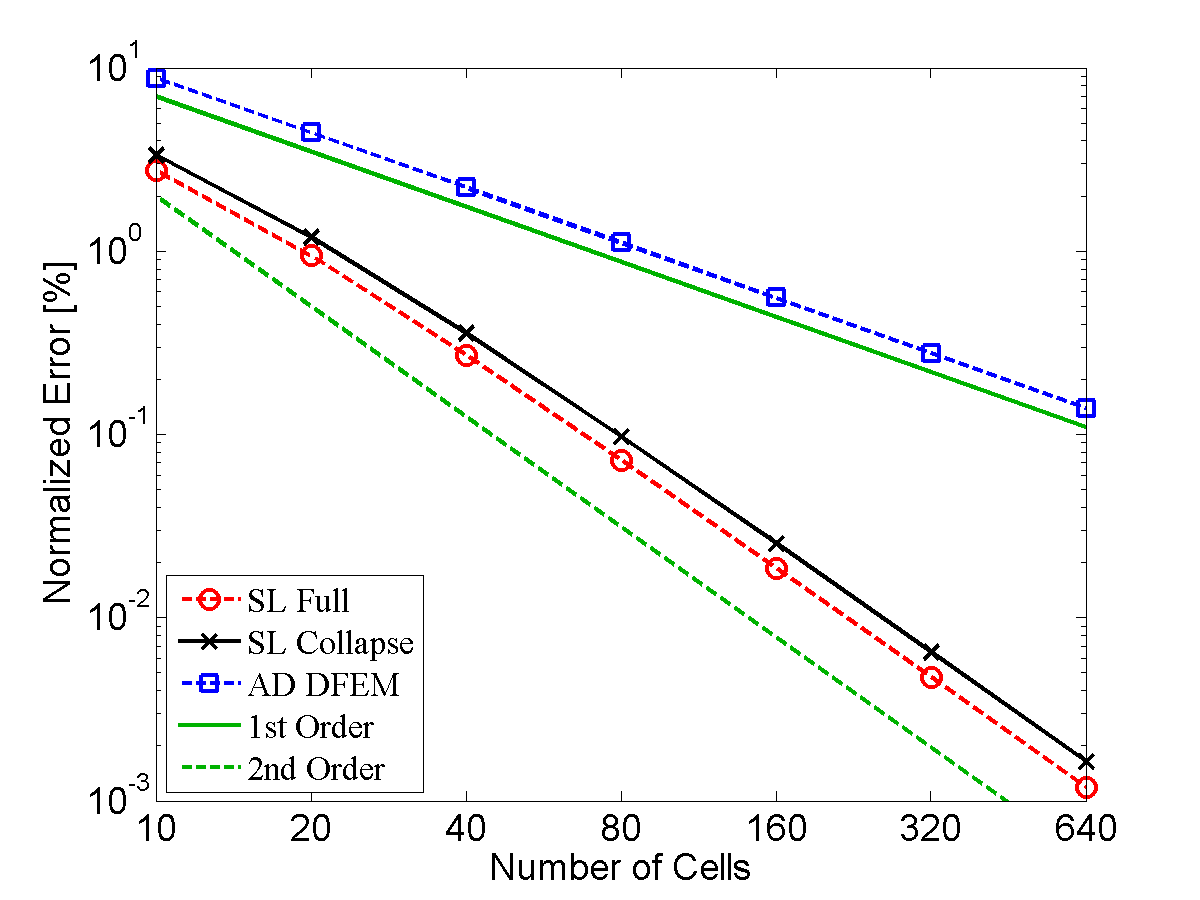
\includegraphics[width=11cm]{chapter5_depletion/FS_P1_norm_err.png}
\caption{Normalized fissile nuclide density error, $E_{N_{FS}}$, for the depletion problem at end of cycle, as a function of angular flux trial space degree.}
\label{fig:depletion_NFS_p1}
\end{figure}

\begin{figure}[!hbp]
\centering
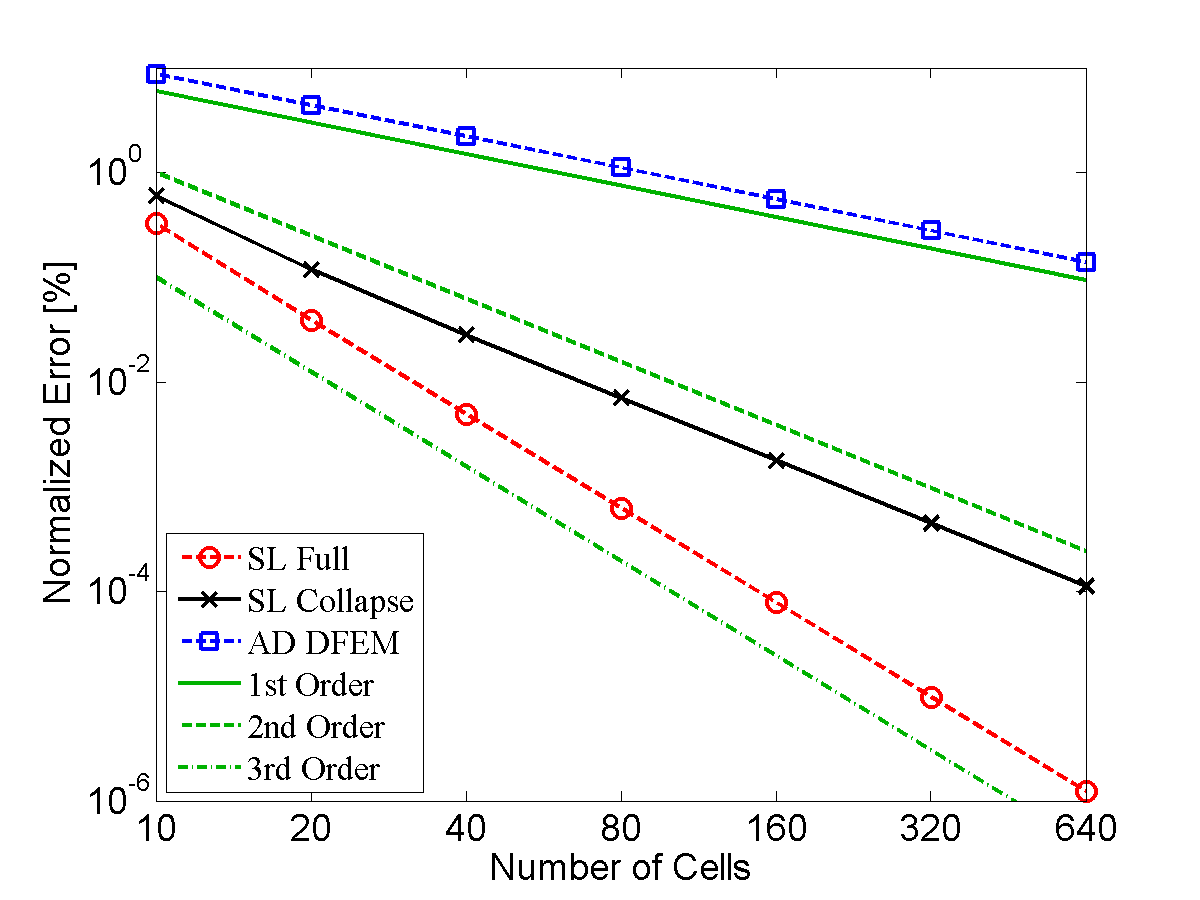
\includegraphics[width=11cm]{chapter5_depletion/FS_P2_norm_err.png}
\caption{Normalized fissile nuclide density error, $E_{N_{FS}}$, for the depletion problem at end of cycle, as a function of angular flux trial space degree.}
\label{fig:depletion_NFS_p2}
\end{figure}

\begin{figure}[!htp]
\centering
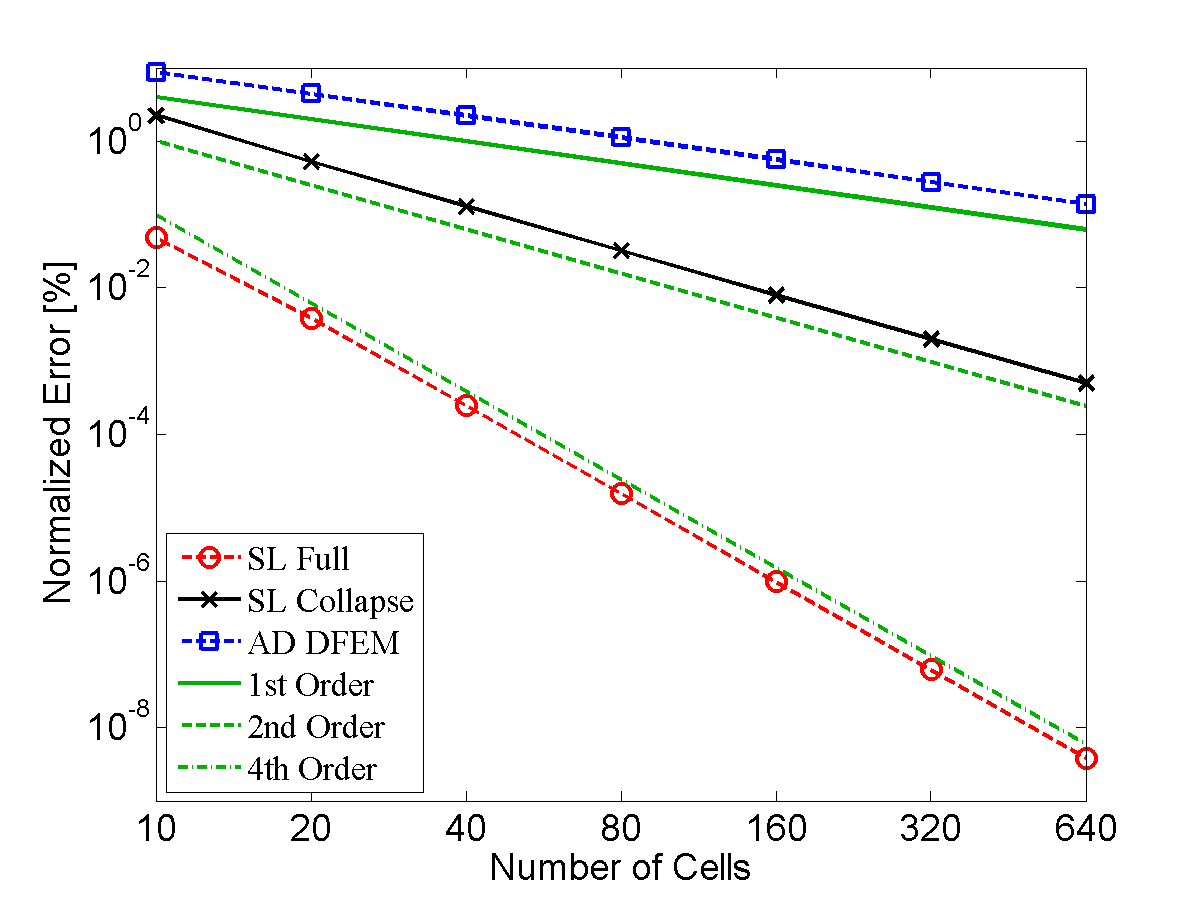
\includegraphics[width=11cm]{chapter5_depletion/FS_P3_norm_err.png}
\caption{Normalized fissile nuclide density error, $E_{N_{FS}}$, for the depletion problem at end of cycle, as a function of angular flux trial space degree.}
\label{fig:depletion_NFS_p3}
\end{figure}

\begin{figure}[!hbp]
\centering
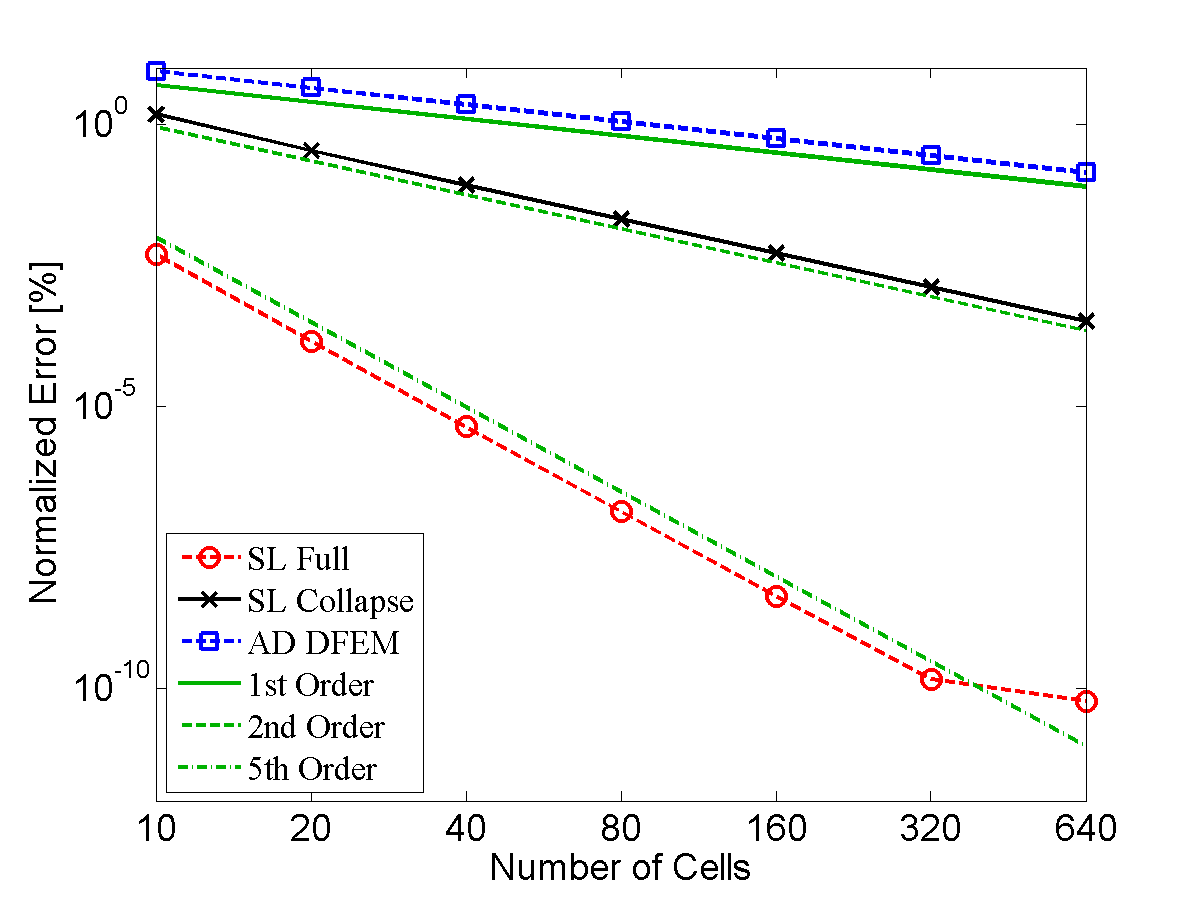
\includegraphics[width=11cm]{chapter5_depletion/FS_P4_norm_err.png}
\caption{Normalized fissile nuclide density error, $E_{N_{FS}}$, for the depletion problem at end of cycle, as a function of angular flux trial space degree.}
\label{fig:depletion_NFS_p4}
\end{figure}

\pagebreak

\begin{figure}[!htp]
\centering
\includegraphics[width=11cm]{chapter5_depletion/ft_P1_norm_err.png}
\caption{Normalized fertile nuclide density, $E_{N_{ft}}$, for the depletion problem at end of cycle, as a function of angular flux trial space degree.}
\label{fig:depletion_NFT_p1}
\end{figure}

\begin{figure}[!hbp]
\centering
\includegraphics[width=11cm]{chapter5_depletion/ft_P2_norm_err.png}
\caption{Normalized fertile nuclide density, $E_{N_{ft}}$, for the depletion problem at end of cycle, as a function of angular flux trial space degree.}
\label{fig:depletion_NFT_p2}
\end{figure}

\begin{figure}[!htp]
\centering
\includegraphics[width=11cm]{chapter5_depletion/ft_P3_norm_err.png}
\caption{Normalized fertile nuclide density, $E_{N_{ft}}$, for the depletion problem at end of cycle, as a function of angular flux trial space degree.}
\label{fig:depletion_NFT_p3}
\end{figure}

\begin{figure}[!hbp]
\centering
\includegraphics[width=11cm]{chapter5_depletion/ft_P4_norm_err.png}
\caption{Normalized fertile nuclide density, $E_{N_{ft}}$, for the depletion problem at end of cycle, as a function of angular flux trial space degree.}
\label{fig:depletion_NFT_p4}
\end{figure}


\pagebreak

\begin{figure}[!htp]
\centering
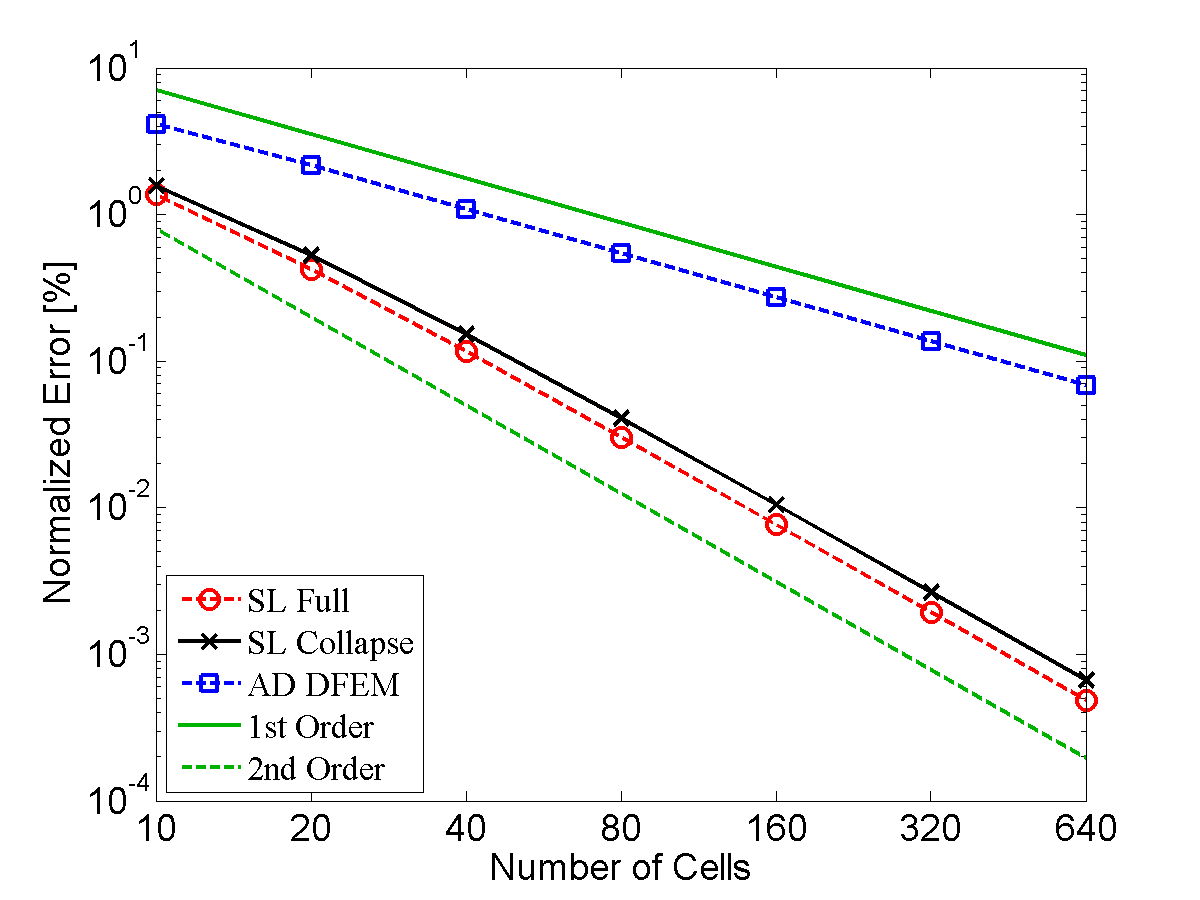
\includegraphics[width=11cm]{chapter5_depletion/FPA_P1_norm_err.png}
\caption{Normalized parasitic absorber fission product error, $E_{N_{FPA}}$, for the depletion problem at end of cycle, as a function of angular flux trial space degree.}
\label{fig:depletion_NFPA_p1}
\end{figure}

\begin{figure}[!hbp]
\centering
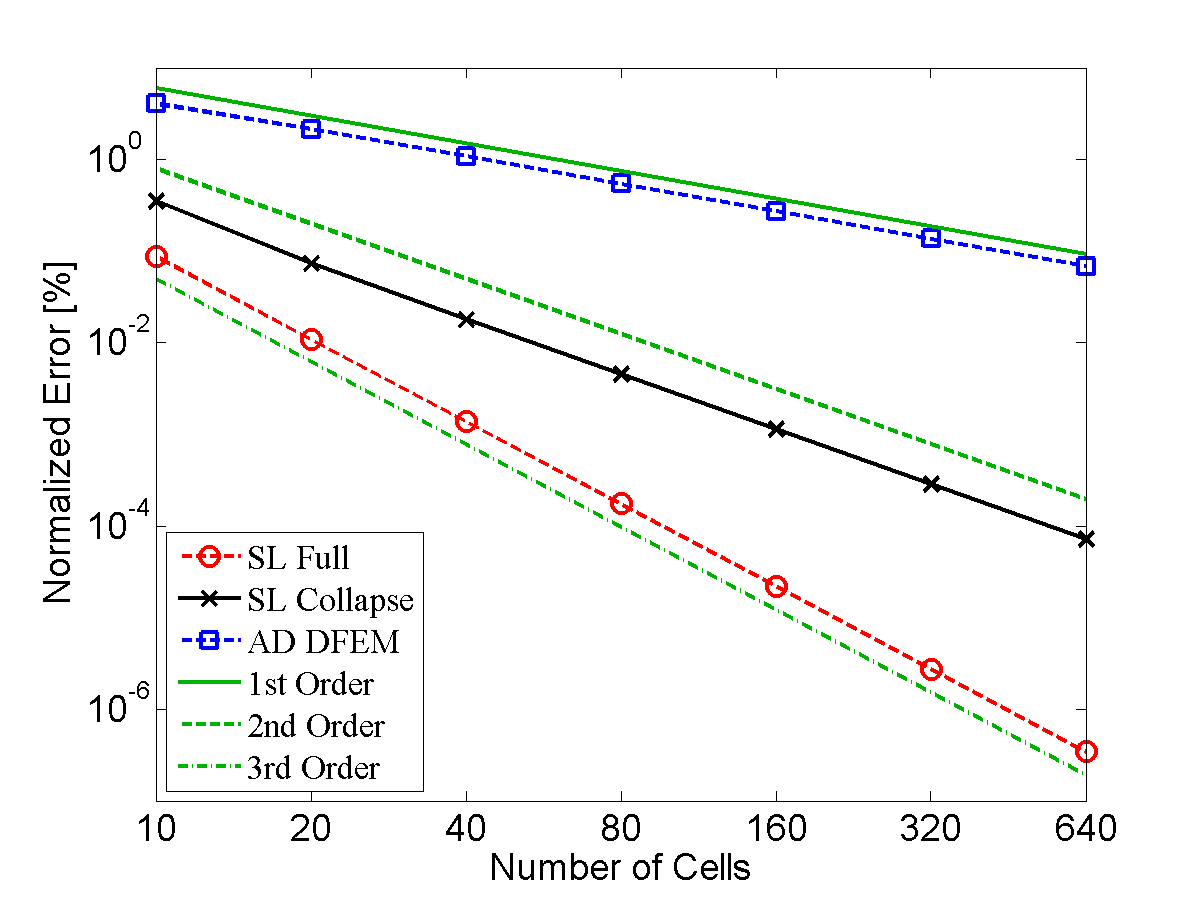
\includegraphics[width=11cm]{chapter5_depletion/FPA_P2_norm_err.png}
\caption{Normalized parasitic absorber fission product error, $E_{N_{FPA}}$, for the depletion problem at end of cycle, as a function of angular flux trial space degree.}
\label{fig:depletion_NFPA_p2}
\end{figure}

\begin{figure}[!htp]
\centering
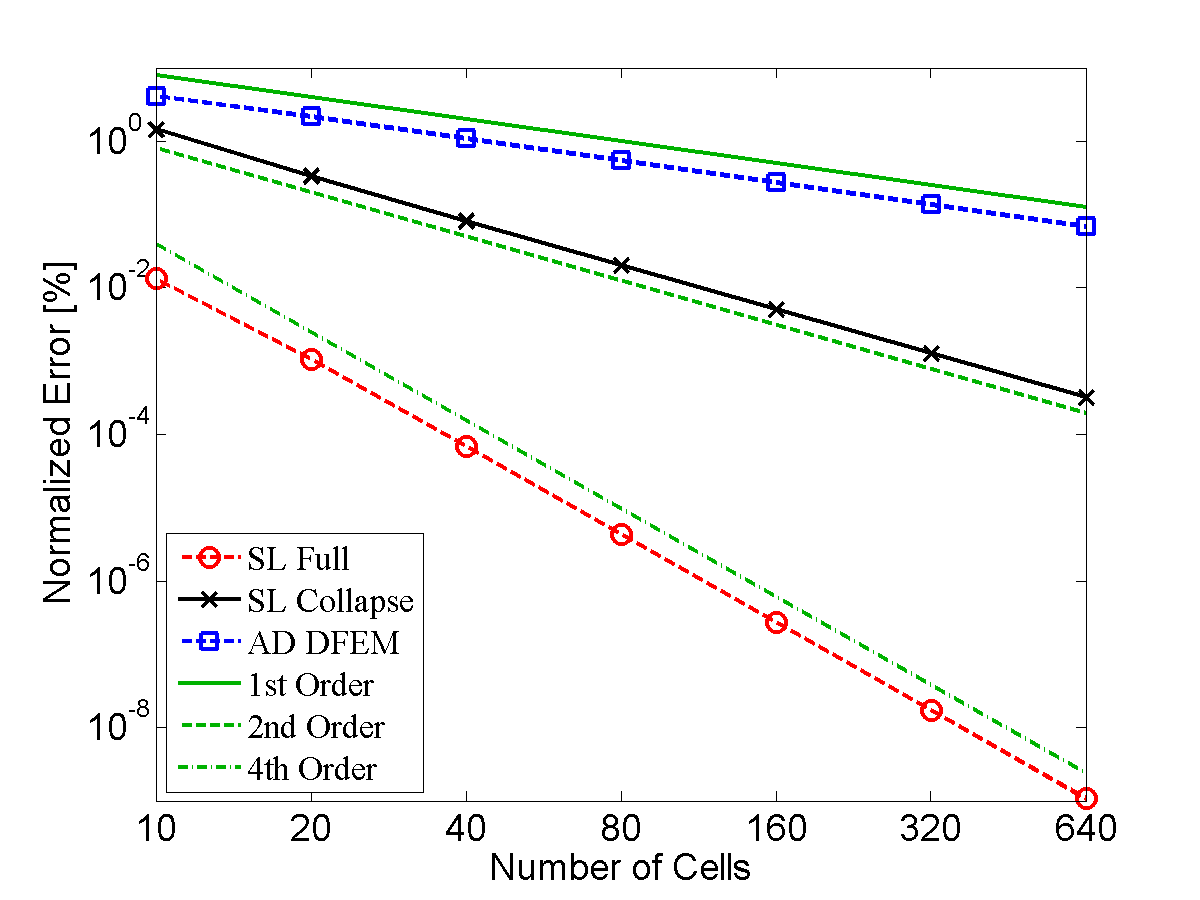
\includegraphics[width=11cm]{chapter5_depletion/FPA_P3_norm_err.png}
\caption{Normalized parasitic absorber fission product error, $E_{N_{FPA}}$, for the depletion problem at end of cycle, as a function of angular flux trial space degree.}
\label{fig:depletion_NFPA_p3}
\end{figure}

\begin{figure}[!hbp]
\centering
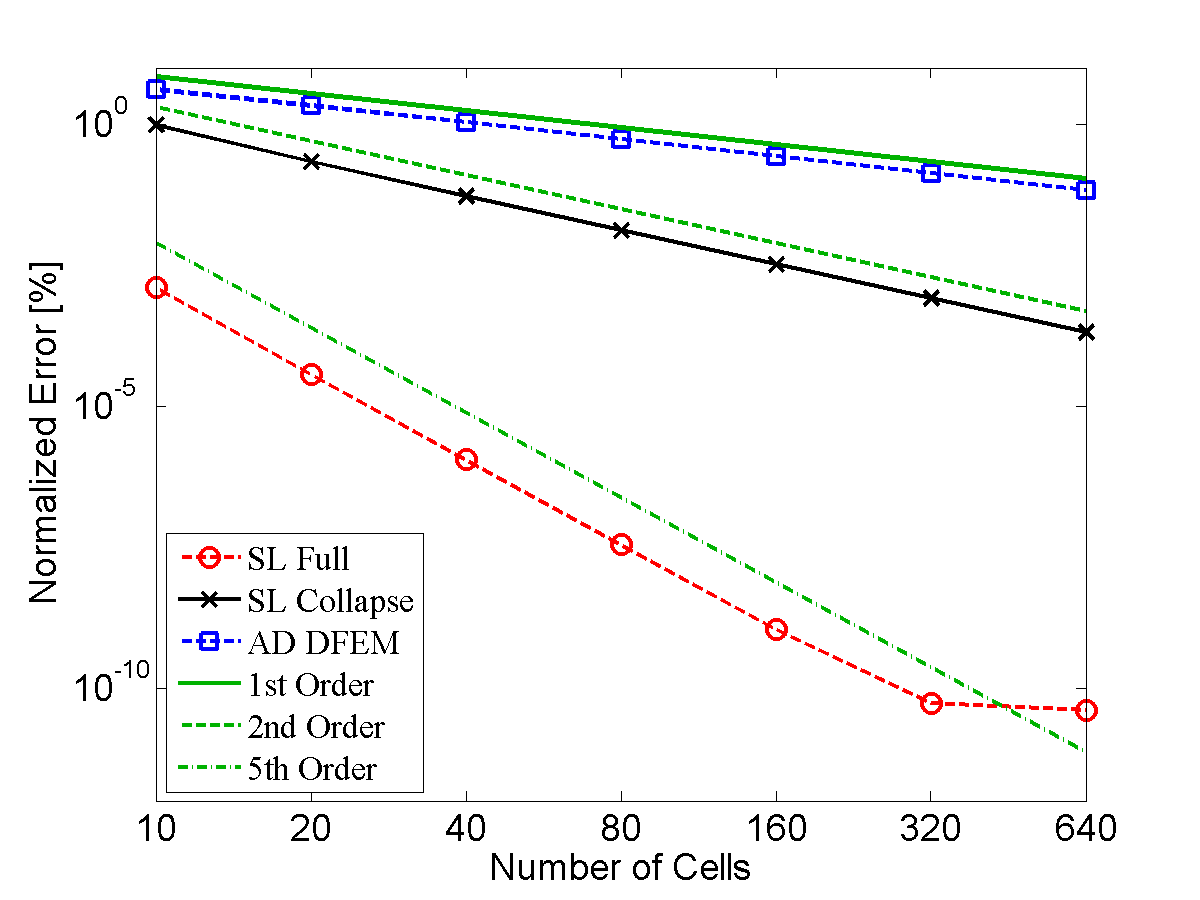
\includegraphics[width=11cm]{chapter5_depletion/FPA_P4_norm_err.png}
\caption{Normalized parasitic absorber fission product error, $E_{N_{FPA}}$, for the depletion problem at end of cycle, as a function of angular flux trial space degree.}
\label{fig:depletion_NFPA_p4}
\end{figure}  
Examining the spatial convergence in nuclide densities, we make several observations.  
First, we note that the AD DFEM scheme (cell-wise average cross section, cell average nuclide density) achieves at most first-order convergence for all spatial nuclide density errors, regardless of the angular flux trial space degree.  
The AD DFEM scheme is limited to at most first-order convergence of the error in the spatial distribution of nuclides because the scalar flux is updated using only a cell-wise average cross section and only the cell average nuclide density is tracked.
Second, though the SL Collapse scheme expands nuclide density in a $P$ degree polynomial DFEM trial space, it achieves at most second-order $L^2$ convergence of the error in nuclides spatial distribution, for all trial  space polynomial degrees.  
SL Collapse is limited to at most second-order convergence of the spatial nuclide density solely because the scheme assumes a constant cross section in each cell when updating the scalar flux.  
The respective first-order and second-order convergence of the error in nuclide spatial distribution of the AD DFEM and SL Collapse scheme verifies the result observed in the pure absorber problem: assuming a cell-wise average cross section for coupled radiation transport problems limits the order of convergence of any quantity that depends on an interaction rate.
SL Full achieves $P+1$ order convergence of the error in spatial nuclide density for the fuel depletion problem, showing that coupled systems of equations involving radiation transport can be solved with arbitrary order of accuracy using high-order DFEM polynomial trial spaces and self-lumping numerical quadrature that explicitly accounts for the spatial variation of cross section within each cell.

